\documentclass[12pt]{elsarticle}

\usepackage{amsmath}
\usepackage{natbib}
\usepackage{enumitem}
\usepackage[T1]{fontenc}
\usepackage[margin=3cm]{geometry}
%\usepackage{biblatex}


\makeatletter
\def\ps@pprintTitle{%
 \let\@oddhead\@empty
 \let\@evenhead\@empty
 \def\@oddfoot{}%
 \let\@evenfoot\@oddfoot}
\makeatother

\begin{document}
\begin{frontmatter}
\title{Using Supervised Learning to Predict Myers-Briggs Personality Types from Text}
\author{Felix Mohr}
\address{Karlsruhe, Germany}

\iffalse
\begin{abstract}
%% Text of abstract
Suspendisse potenti. Suspendisse quis sem elit, et mattis nisl. Phasellus consequat erat eu velit rhoncus non pharetra neque auctor. Phasellus eu lacus quam. Ut ipsum dolor, euismod aliquam congue sed, lobortis et orci. Mauris eget velit id arcu ultricies auctor in eget dolor. Pellentesque suscipit adipiscing sem, imperdiet laoreet dolor elementum ut. Mauris condimentum est sed velit lacinia placerat. Vestibulum ante ipsum primis in faucibus orci luctus et ultrices posuere cubilia Curae; Nullam diam metus, pharetra vitae euismod sed, placerat ultrices eros. Aliquam tincidunt dapibus venenatis. In interdum tellus nec justo accumsan aliquam. Nulla sit amet massa augue.
\end{abstract}
\fi


\end{frontmatter}


\section{Definition}

\subsection{Overview}
\label{subsec:overview}
In his 1921 book \textit{Psychological Types}, Swiss psychoanalyst \textsc{Carl Gustav Jung} developed a theory according to which a person's personality is determined by four dimensions. The four psychological dimensions identified by Jung are
\begin{itemize}
\item \textit{extroversion} vs. \textit{introversion}
\item \textit{intuition} vs. \textit{sensing}
\item \textit{thinking} vs. \textit{feeling}
\item \textit{judging} vs. \textit{perceiving}
\end{itemize}
According to Jung, there exist complex interrelations between different dominant and subdominant personality traits present in a person. The complex character of Jung's theory makes it difficult for a layperson to apply his typology. \textsc{Isabel Briggs Myers} and \textsc{Katharine Briggs}  therefore developed the \textit{Myers-Briggs Type Indicator (MBTI)}, which is based on Jung's theory, yet easier to understand. Although frequently critisized, the MBTI is widely used in various contexts like psychotherapy, self-improvement seminars and human resources.


A person's style of communication often allows us to make accurate assumptions about their personality traits quite easily. If a person's MBTI is a good indication of their personality, we hence can expect their writing style to correlate with the expected writing style of people classified by the same Myers-Briggs indication. To examine whether this assumption holds, we will use data from the \textit{PersonalityCafe} forum\footnote{http://personalitycafe.com/forum} made publicly available via kaggle\footnote{https://www.kaggle.com/datasnaek/mbti-type}. This dataset contains all posts of 8675 users in the personality cafe forum which are labelled with their respective MBT indications. 



\subsection{Problem Statement}
It has been shown by various research projects (e.\,g. \cite{golbeck}, \cite{dutch} and \cite{dl}) that machine learning techniques can be applied to make assumptions about personality based on text data. Identifying the MBTI from text written by a person will allow for several applications, e.\,g. in improving the personalized user experience presented to them on a web application.


In this project, we will therefore apply machine learning techniques to examine whether a person's MBTI correlates with their writing style. If interrelations can be detected, we can -- in opposition to some critics -- conclude that the MBTI in fact is a meaningful indication of a person's personality traits. Our goal is the development of classifiers that are able to identify a person's personality traits from text. This is a challenging problem, as even for a human observer it is not trivial to derive personality traits from written text. Also, our training dataset is not quite large. Taking this into account, we will develop four models -- each of these models categorizes a person according to one of the four personality dimensions described above. We assume that it is possible to derive personality traits in each of the four dimensions from text independently. Considering that even a human reader will not be able to perfectly classify users based on their posts, we expect that the predictions of the developed classifiers will clearly correlate with the true labels, but we can not presuppose classifications that are nearly perfect.



\subsection{Evaluation Metric}
It is our goal to reach a high accuracy in classifying users by the posts they have written. The accuracy is defined as 
\begin{equation}
\nonumber accuracy = \frac{tp + tn}{tp + fp + tn + fn}
\end{equation}

where $tp$ is the number of \textit{true positives}, $tn$ are the \textit{true negatives} etc. I.\,e., the accuracy of a classifier denotes the proportion of objects that are being correctly classified. As we are equally interested in people showing any personality traits, accuracy is the most suitable evaluation metric to the stated problem. To apply this metric, we will have to use balancing techniques in case of unbalanced class labels.


\section{Analysis}
\subsection{Data Exploration}
\label{subsec:exploration}
As mentioned in section \ref{subsec:overview}, the data used for this project consists of the labelled forum posts of 8675 users of the \textit{personality cafe} forum. There exist 16 different class labels, each belonging to one of the 16 possible Myers-Briggs indications. The data has been made available as a CSV file. The first entries of this file can be seen in table \ref{tab:data}. Each row in this file contains the MBTI label of a user together with all of the user's forum posts, which are separated by three pipe characters (|||) respectively. 






\begin{table}[ht]
\centering
\begin{tabular}{| l |l |l |}
\hline
   & \textbf{type} & \textbf{posts} \\
  \hline
  \textbf{0} & INFJ & http://www.youtube.com/watch?v=qsXHcwe3krw|||... \\
  \hline
  \textbf{1} & ENTP & Good one https://www.youtube.com/wat... \\
  \hline
  \textbf{2} & INTP & Dear INTP, I enjoyed our conversation the o... \\
  \hline
  ... & ... & ... \\
  \hline
\end{tabular}
\caption{The available data consists of labelled users, represented by their forum posts.}
\label{tab:data}
\end{table}


The total number of characters written by each forum user\footnote{The separation characters ||| have not been removed prior to performing this analysis.} has a median length of 7515 characters and a mean length of 7235 characters. As can be seen from the boxplot in figure \ref{fig:lengths}, there exist several extreme outliers of users that have written little text. Features created for these users might be less meaningful than features created for users which have written a larger amount of text. Hence, these objects -- of which there exist 179 (2\,\% of the total data) -- will be removed from our dataset in later steps.






\begin{figure}[ht]
\centering
\label{fig:lengths}
\caption{Total lengths of all posts written by the respective forum users in our dataset}
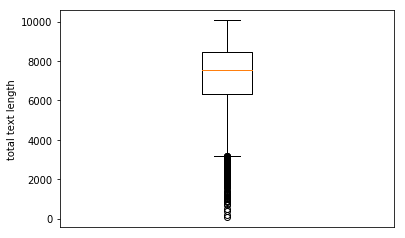
\includegraphics[width=0.5\textwidth]{img/lengths.png}
\end{figure}
When training our classifiers, we will not be using the 16 classes that are available in the initial data. Instead, we will be training independent classifiers, where each classifier learns to distinguish persons in one of the four personality dimensions. Hence, we will be considering 8 classes (\textit{extrovert, introvert, feeling, thinking, ...}).

The two classes for each of the four personality dimensions are not balanced in the available data. Table \ref{tab:classes} denotes the number of available samples for each of the 8 classes after the outliers have been removed.


\begin{table}[ht]
\centering
\begin{tabular}{| l |r |l |}
\hline
  \textbf{type} & \textbf{number} \\
  \hline
  extrovert & 1957 \\
  \hline
  introvert & 6539 \\
  \hline
  intuitive & 7342 \\
  \hline
  sensing & 1154  \\
  \hline
  thinking & 3891 \\
  \hline
  feeling & 4605 \\
  \hline
  percepting & 5132 \\
  \hline
  judging & 3364  \\
  \hline
\end{tabular}
\caption{Labelled users per class}
\label{tab:classes}
\end{table}

\subsection{Algorithms and Techniques}
In this project, we will be using both algorithms of unsupervised and supervised learning. 

\subsubsection{Principal Component Analysis}
The unsupervised algorithm that will be used is \textit{Principal Component Analysis (PCA)}. Textual data often is being processed in the form of \textit{bag-of-words} vectors. This means that first, we have to create a vocabulary $V$ of all the words in our text corpus. In our case, this corpus consists of the total text written by all forum users. $v_i$ is the $i$-th word in our vocabulary. A text document -- in our case, the total posts written by a respective user -- can then be represented by its bag-of-words vector $b$, which has an entry of $n$ at any position $i$ of a word $v_i$ that has been written by this user $n$ times.

These vectors usually will be very high-dimensional. One step that will be used for dimensionality reduction is the application of PCA. PCA performs a transformation of the original vectors in a dataset to a lower-dimensional space. The number of dimensions in the transformed space can be chosen arbitrarily, but too low dimensions might lead to a significant loss of information. The transformation is performed in such a way that the first \textit{principal component} accounts for as much variability as possible in the original space. The subsequent principal components are chosen orthogonal to any other principal component, while ensuring that they keep the maximum amount of variability that is possible under this constraint. Accordingly, the principal component $i$ amounts for more variability in the original data than principal component $j$ if $i < j$, and can therefore be considered to be more meaningful. The number of principal components in the transformed dataspace is usually chosen based on the amount of variability that can be explained by the available principal components cumulatively.




\subsubsection{Stemming}
Another measure we will take to reduce the dimensionality will be \textit{stemming}. Stemming is a standard technique in \textit{Natural Language Processing (NLP)}. Stemming transforms any word in a corpus to its root form -- e.\,g. the word \textit{says} will be transformed to the word \textit{say}. 


\subsubsection{Random Forests}
The \textit{Random Forest (RF)} algorithm is a supervised learning algorithm that will be used to train classifiers. Using a random forest for a classification task, multiple \textit{decision trees} are being trained independently to take decisions about the class of input objects. The prediction will be the class that has been chosen by the majority of independent classifiers. RFs hence are a \textit{bootstrap aggregation (bagging)} algorithm. We will be using Random Forests as they have several advantages compared to other classification algorithms. Firstly, Random Forests are faster than comparabled algorithms like \textit{Support Vector Machines (SVMs)}. Another advantage is that they allow us to easily examine which features are most meaningful for performing classifications. I.\,e. this might allow us to understand which words are most distinctive for comparing extroverted and introverted persons etc.

Applying a random forest requires the choice of multiple parameters. Parameters that we will be going to adjust are the following:
\begin{itemize}
\item The number of independent decision tree classifiers
\item The minimum number of samples per leaf in any decision tree
\item The minimum number of samples to perform a split for any decision tree
\end{itemize}

\subsubsection{Grid Search}
The technique we will be applying for parameter optimization is called \textit{grid search}. The parameters that our classifier will be trained with often are interrelated. Therefore, they can not be chosen independently. When performing grid search, for any chosen parameter a list of test values is created. Classifiers with any possible combination of parameter values from the lists will be trained; the classifier performing the best is being kept.


\subsubsection{Undersampling}
Undersampling is a method for class balancing. As has been mentioned in \ref{subsec:exploration}, classes for each of the four personality dimensions are not balanced (see figure 2). Unbalanced classes can lead to decreased classification performance. We hence perform a technique called \textit{undersampling}. In each of the four personality dimensions, we have two classes $C_1$ and $C_2$, without loss of generality we have $|C_1|=n_1>|C_2|=n_2$. We now remove $n_1-n_2$ randomly chosen samples that are labelled with the first class to balance our dataset.





\begin{figure}[ht]
\label{fig:pies}
\caption{Relative amount of users per class.}

\vspace{1em}
\centering
\begin{minipage}{0.48\textwidth}
  \centering
  \frame{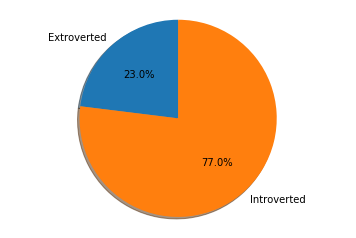
\includegraphics[width=.9\linewidth]{img/pie_ie.png}}
\end{minipage}
\begin{minipage}{0.48\textwidth}
  \centering
  \frame{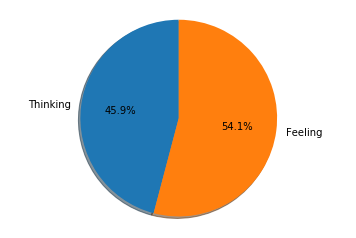
\includegraphics[width=.9\linewidth]{img/pie_tf.png}}
\end{minipage}

\vspace{1em}

\begin{minipage}{0.48\textwidth}
  \centering
  \frame{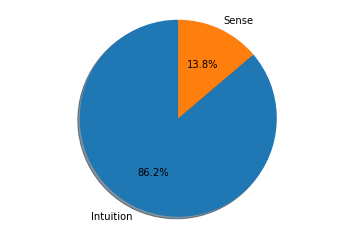
\includegraphics[width=.9\linewidth]{img/pie_ns.png}}
\end{minipage}
\begin{minipage}{0.48\textwidth}
  \centering
  \frame{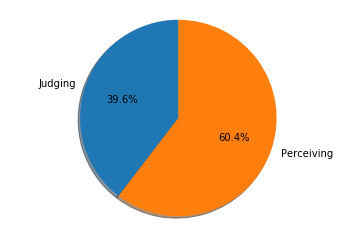
\includegraphics[width=.9\linewidth]{img/pie_jp.png}}
\end{minipage}
\end{figure}






\subsection{Exploratory Visualization}
We assume that comparing the word2vec means of the texts written by each user will allow us to distinguish them based on their Myers-Briggs indications. To examine whether a strong correlation exists, PCA has been applied to reduce the dimensionality of each user's mean \textit{word2vec} vector to two dimensions, and the results have been visualized (see figure 3 on page \pageref{fig:viz}). 


Two dimensions don't seem to allow for a separation of the different personality traits. However, the first two PCA dimensions account for only 30\,\% of the total variance in the untransformed data, and the word2vec representations may still be useful.


\begin{figure}[ht]
\label{fig:viz}
\caption{Visualization of the posts of 300 users per class and plot -- the axis labels have been removed as irrelevant (PCA components can not be intuitively interpreted).}

\vspace{1em}
\centering
\begin{minipage}{0.48\textwidth}
  \centering
  \frame{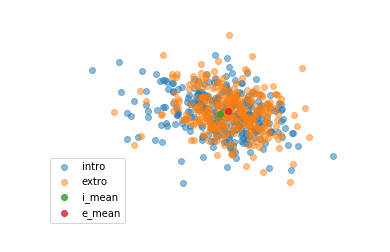
\includegraphics[width=.9\linewidth]{img/viz_ie.png}}
\end{minipage}
\begin{minipage}{0.48\textwidth}
  \centering
  \frame{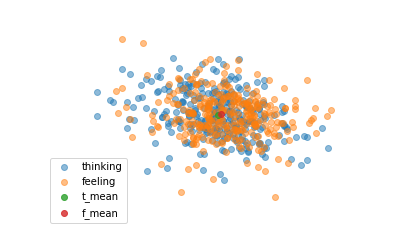
\includegraphics[width=.9\linewidth]{img/viz_tf.png}}
\end{minipage}

\vspace{1em}

\begin{minipage}{0.48\textwidth}
  \centering
  \frame{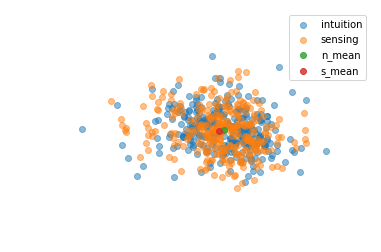
\includegraphics[width=.9\linewidth]{img/viz_ns.png}}
\end{minipage}
\begin{minipage}{0.48\textwidth}
  \centering
  \frame{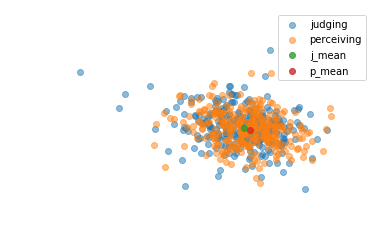
\includegraphics[width=.9\linewidth]{img/viz_jp.png}}
\end{minipage}
\end{figure}



\clearpage



\subsection{Benchmark}
To create a simple benchmark model, we perform the following steps:
\begin{enumerate}
\item Any mentionings of personality types \textit{ISTP, ...} were removed from the text.
\item For any of the four personality dimensions, we use undersampling for class balancing.
\item We perform a stemming of all posts, we remove special characters.
\item We create a vocabulary. The vocabulary consists only of the words that appear more than 500 times and has a size of 1619 words.
\item Every user is being transformed to a bag-of-words representation, which is a 1619-dimensional vector that denotes the words that have been written by this user and the number of occurences of these words in the user's posts.
\item Now four unoptimized Random Forest classifier with $10$ decision tree estimators are being trained to distinguish users in any of the four personality dimensions.
\end{enumerate}
This way, we achieve a better classification accuracy than if we had used random guessing (expected accuracy of $50\,\%$). The accuracies in the four dimensions are the following:
\begin{itemize}
\item Introversion vs. extroversion: $58.1\,\%$
\item Intuition vs. sensing:  $56.1\,\%$
\item Thinking vs. feeling:  $62.3\,\%$
\item Judging vs. perceiving:  $54.2\,\%$
\end{itemize}
We can conclude that it is in fact possible to derive MBTI personality traits from writing style, even without any optimization steps. 


\newpage
\section{Methodology}
\subsection{Data Preprocessing}
\label{subsec:preprocessing}
Firstly, outliers based on text length were removed (see \ref{subsec:exploration}). Also, any mentionings of personality types \textit{ISTP, ...} were removed from the text. Then, undersampling was performed to create an equal number of samples for both classes of any of the four personality dimensions. I.\,e. after having performed undersampling, we have 1957 extroverted and 1957 introverted samples; 1154 sensing and 1154 intuitive samples etc. Afterwards, we created training and testing sets. The latter will be used in later steps for calculating generalization errors. In each of the 8 classes, 25\,\% of samples were randomly chosen to create the respective test set. The remaining 75\,\% will be used for training.


Now, all training and testing samples were transformed to three different vector representations, which will be discussed in the following subsections.

\subsubsection{Bag-of-Words}
To create bag-of-words vectors, the same steps have been performed as in the creation of the benchmark classifiers: All posts were stemmed, special characters were removed and a vocabulary of the words that appeared at least 500 times was created, leading to a dimensionality of 1619. Now, for any sample we created a vector which denotes for each word the number of occurences in the respective user's text.

\subsubsection{Word2Vec}
We also represent every data object by its representation in a 300-dimensional Word2Vec dataspace. To this end, we used Word2Vec vectors that have been pretrained by Google on part of the Google News dataset\footnote{https://code.google.com/archive/p/word2vec/}. We build on the findings made by the authors of \cite{wmd}. The authors develop the \textit{word mover's distance} as a means to compare different documents for their similarity. To accomplish this, every document is represented by the mean of its word2vec vectors, and documents are considered more similar if their respective means are less distant, compared by the Euclidean distance. 


We represent users in our dataset by the mean of the word2vec representation of the words written by them. Due to technical limitations\footnote{Available RAM was insufficient to work with more vectors.}, we only consider the 1\,200\,000 most frequent words in the model that was pretrained by Google. Before transforming the words, special characters were removed. 


\subsubsection{Hand-crafted Features}
We also developed some additional features that may be helpful in identifying personality traits.  Every data sample is being transformed to a vector with entries denoting the values of the following features:

\begin{itemize}
\item Relative occurence of pronouns in text written by the user, as compared to the other three parts-of-speech that are being considered
\item Relative occurence of space characters in text written by the user, as compared to the other three parts-of-speech that are being considered
\item Relative occurence of verbs in text written by the user, as compared to the other three parts-of-speech that are being considered
\item Relative occurence of adverbs in text written by the user, as compared to the other three parts-of-speech that are being considered
\item Occurences of the string \textit{http} per post
\item Occurences of question marks (\textit{?}) per post
\item Occurences of exclamation marks (\textit{!}) per post
\item Occurences of periods (\textit{.}) per post
\item Occurences of colons (\textit{:}) per post -- these are sometimese being used to denote emoticons 
\item Average number of words per post
\end{itemize}




\subsection{Implementation}
For each of the four personality dimensions, we each trained a total of four different classifiers (in total, we created 16 classifiers). For each dimension, one classifier was trained using bag-of-words features; one classifier was trained using word2vec features; one classifier was trained using the hand-crafted features; one classifier was trained using vectors that contained all of the mentioned features. In each case, the training was performed similarly:
\begin{enumerate}
\item We defined values for performing a grid search to optimize a Random Forest classifier. The available parameters were the following:
\begin{itemize}
\item Number of estimators: 50, 60, 80
\item Minimum samples per leaf: 2, 4, 7, 10
\item Minimum samples to perform a split: 3, 5, 7, 9
\end{itemize}
\item A grid search was performed to create an optimized Random Forest classifier for distinguishing extroverted from introverted persons.
\item The parameters of this optimized classifier were taken to train new RF classifiers for the three remaining personality dimensions.
\end{enumerate}



\subsection{Refinement}
We tried applying PCA for dimensionality reduction of the word2vec and bag-of-words vectors. We expected that training classifiers on the transformed data objects might possibly lead to improved performance. However, this assumption could not be confirmed.


In case of the bag-of-words vectors, the dataspace was transformed from having 1619 dimensions to a dataspace of the first 350 principal components. This reduced dataspace still contained $> 90\,\%$ of the original variance available in the data. Using grid search, an optimized RF classifier was trained to distinguish extroverted from introverted users. Performance was worse than performance of the classifier using the untransformed dataspace ($0.622$ vs. $0.570$ accuracy. 


Similarly, the word2vec dataspace was reduced from 300 dimensions to the first 50 principal components, which still accounted for $> 80\,\%$ of the original variance. An RF classifier for distinguishing extroverted from introverted users was trained in a similar manner as in case of the bag-of-words vectors. This classifier did not perform worse than the classifier using untransformed data. However, the improvement was too small to be considered significant ($0.627$ vs. $0.630$ accuracy).


As our approach for refinement did not work out, we continued using the classifiers that were trained on the untransformed data.



\section{Results}
\subsection{Model Evaluation and Validation}
In the process of this project, several models have been trained. Tables \ref{tab:res} shows the results that have been achieved using different feature sets. The best results have been achieved using classifiers trained on the features that were combined over all of the three feature categories that were used. To make sure that the results shown conform to the generalization error, these results have been calculated on the testing data (see \ref{subsec:preprocessing}).


\begin{table}[ht]
\caption{Multi-column table}
\begin{center}
\begin{tabular}{l | l | l | l | l | l }
    \hline
    \multicolumn{6}{c}{\textbf{Individual Features}}\\
    \hline
    \textbf{Feature}  & \textbf{I/E} & \textbf{S/N}&\textbf{T/F}&\textbf{J/P}& \textbf{Average}\\
    {Bag-of-Words} & 62.2\,\%& 65.8\,\%& 73.2\,\%& 60.9\,\%& 65.5\,\% \\
	{Word2Vec}& 62.7\,\%& 65.6\,\%& 73.3\,\%& 60.5\,\%    & 65.5\,\%\\
    {Hand-Crafted}& 54.0\,\%& 51.2\,\%& 61.8\,\%& 52.9\,\%  & 55.0\,\% \\
    \hline
    \multicolumn{6}{c}{\textbf{Combined Features}}\\
    \hline
                  & 64.1\,\%& 67.0\,\%& 72.9\,\%& 61.8\,\%& 66.5\,\% \\
    \hline
\end{tabular}
\end{center}
\label{tab:res}
\end{table}

The parameters that have been used by the final model, using combined features, are the following:
\begin{enumerate}
\item Number of estimators: 80
\item Minimum number of samples per leaf: 7
\item Minimum number of samples for performing a split: 5
\end{enumerate}


Interestingly, prediction accuracy for distinguishing users based on the fourth dimension (J/P) has been lowest for any of the used features. This could possibly be due to the fact that the amount of training data used in this dimension has been the lowest (see figure 2).





\subsection{Justification}
The results that have been achieved align well with our expectations. Even for a human reader, making predictions about personality traits from text is a hard task. Achieving an average accuracy of nearly $\frac{2}{3}$ hence is a satisfactory result. The results of the benchmark models have been improved significantly. The following improvements in accuracy have been achieved in the four personality dimensions:
\begin{itemize}
\item I/E: 10.3\,\% of the benchmark accuracy
\item S/N: 19.4\,\%
\item T/F: 17.0\,\%
\item J/P: 14.0\,\%
\end{itemize}






\clearpage
\section{Conclusion}
\subsection{Free-From Visualization}
\begin{figure}[ht]
\label{fig:words}
\caption{Most distinctive words}

\vspace{1em}
\centering
\begin{minipage}{0.48\textwidth}
  \centering
  {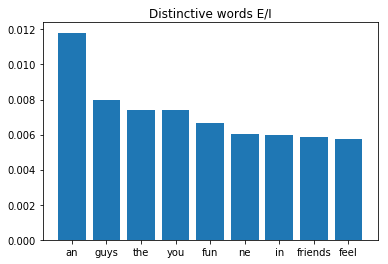
\includegraphics[width=.9\linewidth]{img/words_ie.png}}
\end{minipage}
\begin{minipage}{0.48\textwidth}
  \centering
  {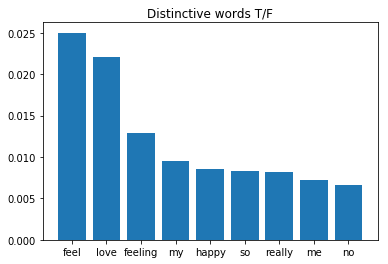
\includegraphics[width=.9\linewidth]{img/words_tf.png}}
\end{minipage}

\vspace{1em}

\begin{minipage}{0.48\textwidth}
  \centering
  {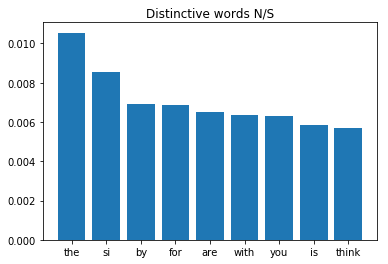
\includegraphics[width=.9\linewidth]{img/words_ns.png}}
\end{minipage}
\begin{minipage}{0.48\textwidth}
  \centering
  {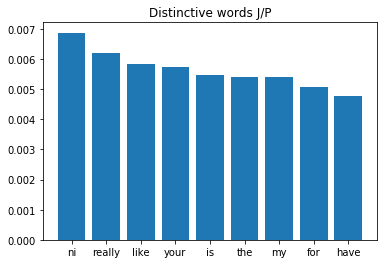
\includegraphics[width=.9\linewidth]{img/words_jp.png}}
\end{minipage}
\end{figure}
To examine the most distinctive words for each of the four personality dimensions, we visualize the feature importances of the random forest classifiers trained on the bag-of-words representations (figure 4). The results seem quite reasonable. E.\,g., we can expect an extroverted person to be more likely to use words like \textit{guys} or \textit{fun} than an introvert; a person labelled as a \textit{feeling} type might more often use words like \textit{love}, \textit{feel} etc. than a thinking character. In case of some words, the influence of personality types on their usage is less obvious, and some of these words might be the result of mere chance.



\subsection{Reflection}
In this project, we developed classifiers for deriving a person's personality traits by analyzing the text written by them. To achieve this, we used three types of features:
\begin{itemize}
\item Bag-of-words features
\item Word2Vec based means, following the approach of the authors of the \textit{word mover's distance}
\item Hand-crafted features, including part-of-speech tags and the relative occurence of various special characters
\end{itemize}
Comparing the results of the trained classifiers, features of the two firstly mentioned categories were more distinctive than the features in the third category. The best results were obtained by training classifiers on the combined features of all three categories.


Taking our results into consideration, we assume that a person's writing style indeed allows for making accurate guesses about their personality traits -- the average accuracy per personality dimension achieved by our classifiers is $\frac{2}{3}$. It is important to note that all training and testing data has been taken from a forum where personality types are being discussed. An interesting further step would be the examination whether personality traits can be identified with an equal accuracy from text that has been written in different domains.





\subsection{Improvement}
In preprocessing, any mentions of personality types (like \textit{ESTJ}) has been removed from the textual data. However, mentions of the cognitive functions\footnote{https://en.wikipedia.org/wiki/Jungian\_cognitive\_functions} like \textit{Te}, \textit{Ni} have not been removed. As can be seen from the word importances in the N/S and J/P dimensions, it seems like these words had an effect on the trained classifiers. The posts analyzed in this project were taken from a forum which is concerned with discussing personality types, and in standard text we can not usually expect mentions of cognitive functions to be present. As an improvement, these words should be removed from our training data. We expect the calculated test accuracies to diminish slightly.

Another possible improvement could be achieved with applying classification algorithms apart from Random Forest classifiers. Whether this would lead to improved accuracies has to be examined experimentally.











\clearpage
\section{References}
\bibliographystyle{plainnat}
\bibliography{lib}

\end{document}
